
 \subsection{Discrete Particle Model}
 Discrete Particle Model simulates particle motion by applying forces and torques which derives from particle-particle interactions and external influences, on the basis of the given contact law. It performs calculations of kinematics that a given particle $i$ exerts on other particle $j$, for each particle in the system, among with the peripheral factors such as gravity and walls. To achieve this results, the particles are assumes to be (1) undeformable - deform therefore implemented as overlap, (2) unbreakable, (3) all internal interactions are due to particle-particle interaction, (4) Each particle pair $i, j$ has only on/viewer.htmle contact point $c_{ij}$ which the forces and torques act on, and (5) all external forces and torques are either body forces and torques or by interacting with a wall~\cite{MercuryDPM}. 

\subsubsection{Contact Laws}
For each particle $i$ on the system, Eq. \ref{eq:force} describes the internal and external forces, and Eq.~\ref{eq:torque} describes the torque acting on it \cite{MercuryDPM}:

\begin{equation} \label{eq:force}
    F_i = \sum_{j=1}^{n_p} F_{ij} + \sum_{k=1}^{n_w} F_{ik}^w  + F_i^b
\end{equation}

\begin{equation} \label{eq:torque}
    \tau_i = \sum_{j=1}^{n_p} r_{ij}F_{ij} + \tau_{ij} + \sum_{k=1}^{n_w} r_{ik}F_{ik}^w + \tau_{ik}^w +\tau_{i}^{b} 
\end{equation}

With $F_{ij}$ interparticle forces, $F_{ik}^w$ the interaction force between each wall and the particle, $n_p =$ number of particles, $n_w =$ number of walls, $F_i^b$ body forces i.e., gravity, and $r_{ij}$ as the branch vector, which connects the particle position $r_i$ with the contact point $c_{ij}$ . The same hold for torques equation, with $\tau$ as torque. 

The contact law used in the simulations is the Linear Spring-Dashpot model, which is implemented in MercuryDPM as 
\texttt{LinearViscoelasticFrictionReversibleAdhesiveSpecies}. It defines the interaction between two particles $i$ and $j$ as a damped harmonic oscillators \cite{LSD-info}:

\begin{equation}
    F_{ij}^n=\begin{cases}
        k_n \delta_{ij}^n + \gamma_n v_{ij}^n &\text{if } \, \delta_{ij}^n > 0, \\
        0 \quad &\text{else, } \,   \\
   \end{cases}
\end{equation}

In this equation, $k_n > 0$ represents spring stiffness, $\gamma_n \geq 0$ represents the damping coefficient, $v_n$ the normal vector, and $\delta_{ij}^n$ is the overlap between the particles. Two particles interact with each other if and only if they overlap. This contact model is simple, has an analytic solution and less computationally expensive \cite{NAVARRO2013}, while also suitable for large particles \cite{MercuryDPM}. 


\subsubsection{Angle of Repose measurement}

In MercuryDPM, Static AoR is measured by a hollow cylinder simulation, which consists of two cylinders (instead of one cylinder and one plate in Fig.~\ref{fig:StaticAoR}), with the cylinder's diameter. For simplicity, all particles in the simulation are assumed to be a perfect sphere. After all the particles are poured into the cylinder, it is let to rest until the bulk's kinetic energy is less than $1\%$ compared to the potential energy (steady-state condition). At this point, the top cylinder is removed, and all the particles that have fallen out of the bottom cylinder below $z = 0$ are deleted. This will result in a cone-shaped heap of particles and a drastic increase in kinetic energy due to gravity. The heap will be rested again until it reach a steady-state condition as mentioned above, and then Static AoR can be measured. The measurement will be done twice, since the kinetic energy of the system can be increased again after the first measurement. Figure~\ref{fig:MercuryAoR} demonstrates an example simulation on MercuryDPM.    



\begin{figure}[H]
    \centering
    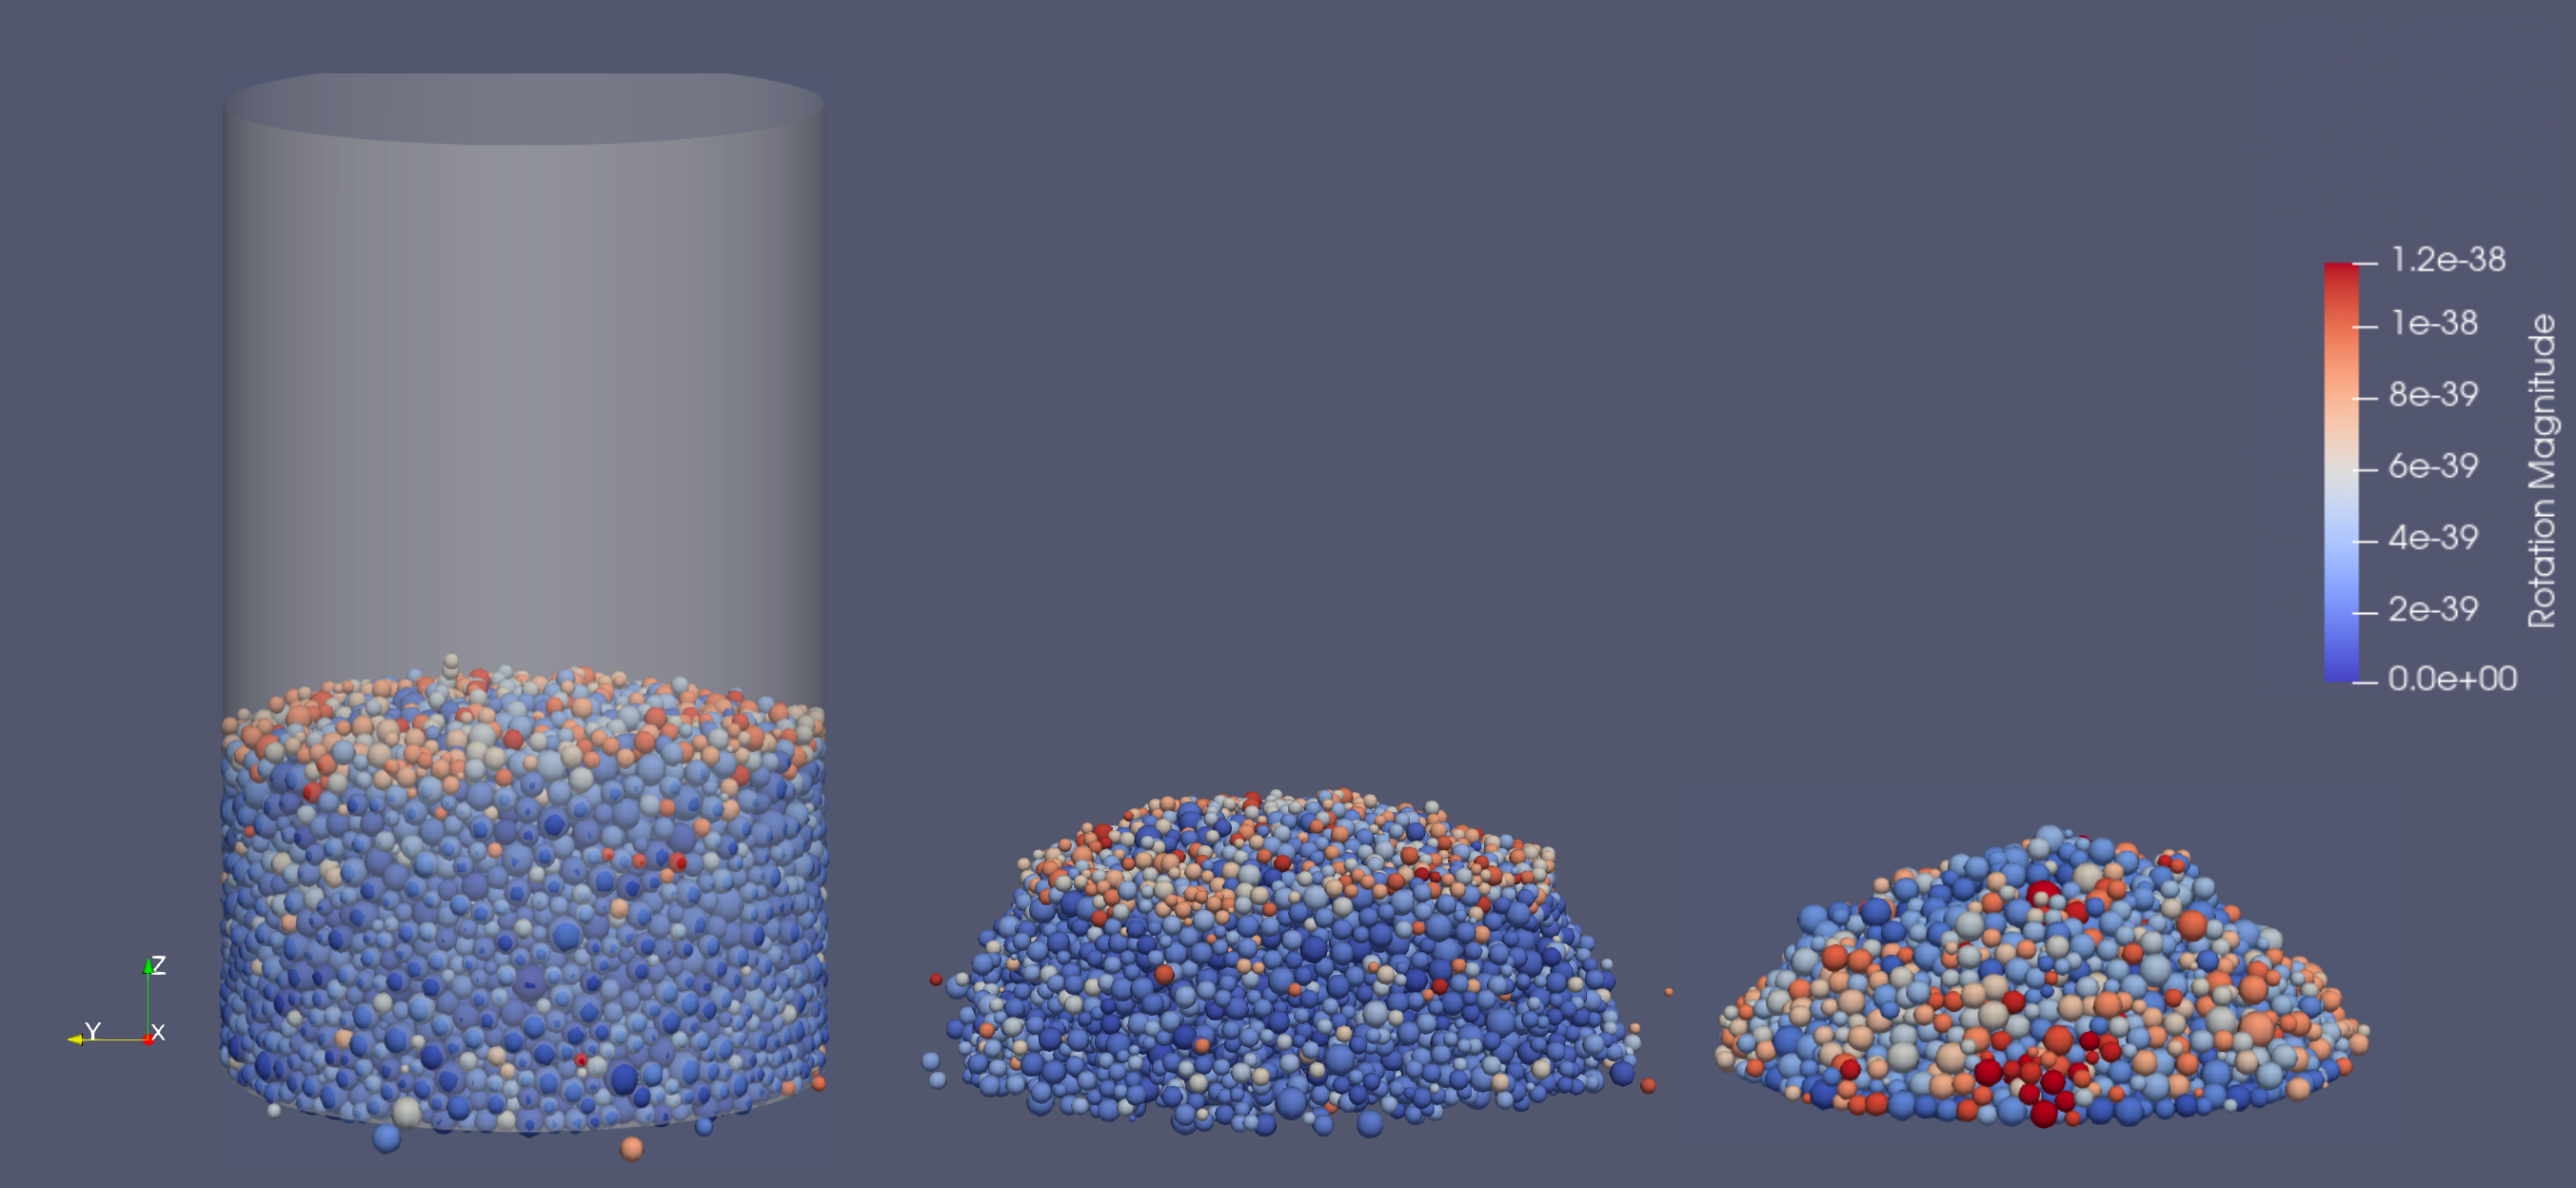
\includegraphics[scale=0.16]{AoRSim.png}
    \caption{Angle of Repose simulation on MercuryDPM. From left to right: Initial fill stage, wall removed, and final stage.}\label{fig:MercuryAoR}
\end{figure}
